\documentclass[12pt,a4paper]{article}
\usepackage[utf8]{inputenc}
\usepackage{amsmath,amsthm, amssymb}
\usepackage{amsfonts}
\usepackage{amssymb}
\usepackage{graphicx} % For pictures
\usepackage[export]{adjustbox}
\usepackage{pdfpages} % for pdfs
\usepackage{listings}
\usepackage{xcolor}
\usepackage{caption}

\definecolor{mGreen}{rgb}{0,0.6,0}
\definecolor{mGray}{rgb}{0.5,0.5,0.5}
\definecolor{mPurple}{rgb}{0.58,0,0.82}
\definecolor{backgroundColour}{rgb}{0.95,0.95,0.95}

\lstdefinestyle{CStyle}{
	backgroundcolor=\color{backgroundColour},   
	commentstyle=\color{mGreen},
	keywordstyle=\color{magenta},
	numberstyle=\tiny\color{mGray},
	stringstyle=\color{mPurple},
	basicstyle=\footnotesize,
	breakatwhitespace=false,         
	breaklines=true,                 
	captionpos=b,                    
	keepspaces=true,                 
	numbers=left,                    
	numbersep=5pt,                  
	showspaces=false,                
	showstringspaces=false,
	showtabs=false,                  
	tabsize=2,
	language=C
}
\lstset{style=CStyle}
\usepackage{titling}
\usepackage[margin=0.75in]{geometry}
\setlength{\droptitle}{-7em}   % This is your set screw
\date{}
\setlength{\parindent}{0em}

\author{Lara Quitte, Tino Jeromin}
\title{Versuch A: Buffer Overflow}


\begin{document}
	\maketitle
	
	
	\section*{Stichwörter}
	Die folgenden Begriffe sind notwendig für den Versuch zu definieren:
	\begin{itemize}
		\item Format String Attack
		\item printf( ) (die C-Funktion)
	\end{itemize}
	
	Diese, sowie weitere wichtige Begriffe, sollen im Folgenden kurz definiert werden.
	\bigskip
	
	\textbf{Format String Attack} \\
	Format String Attacks bezeichen eine Sicherheitslücke in der Programmierung, bei der Angreifer ein Programm zum Absturz bringen, aber auch potentiell schädlichen Code auszuführen können.
	Es handelt sich hierbei nicht um Sicherheitslücken im klassischen Sinne, viel eher ist es bei Format String Attacks möglich sich Bugs im Code zu Nutze zu machen.
	\bigskip
	
	\textbf{printf( )} \\
	Die printf( )- Funktion ist eine Ausgabefunktion, welche ihren Ursprung in der Programmiersprache C hat. Die Funktion gehört zu den Format Funktionen, welche  eine variable Anzahl von Argumenten als Eingabewerte entgegen nehmen. Einer dieser Werte ist der sogenannte Format String. Dieser ist ein ASCIIZ String, welcher sowohl Text als auch Format Parameter enthält, welche wiederum in der Ausgabe mit einem Wert ersetzt wird. Der Format Parameter gibt an, um welche Art von Ausgabe es sich handelt, beispielsweise Dezimalzahlen oder auch Strings.
	\bigskip
	
	\textbf{Format Funktion} \\
	Eine Format Funktion ist eine ANSI C Funktion, wie \textit{printf( )}, die eine primitive Variable der Programmiersprache in eine, vom Menschen lesbare, String Repräsentation konvertiert.
	\bigskip
	
	\textbf{Format String} \\
	Ein Format String ist ein Argument der Format Funktion und besteht aus einem ASCIIZ String, welcher sowohl Text, als auch Format Parameter enthält.
	\bigskip
	
	\textbf{Format String Parameters} \\
	Ein Format String Parameter definieren den Typ der Umwandlung in einer Format Funktion.
	\bigskip

	
	\section*{Teil 2: Format String Attack}
	
	\textbf{Fragestellung: Wie funktioniert eine Format String Attack grundsätzlich?} \\
	Bei der Format String Attack macht sich der Angreifer eine fehlerhafte Implementation der \textit{printf( )-Funktion} zu Nutze. Wird in dieser kein Format String angegeben, so ist es möglich diese Schwachstelle auszunutzen, indem man einen String übergibt, der gültige \textbf{Format-Parameter} enthält. Diese werden dann als \textit{Format String} interpretiert und ausgeführt, wodurch vom Speicher gelesen wird, was der Angreifer schadhaft ausnutzen kann. Die \textit{Format Funktion} ließt dann einfach die nächsten Daten des Speichers, wodurch es zum Kontrollverlust über den Prozess kommen kann.
	\bigskip
	
	Um den zweiten Teil des Versuches durchzuführen, haben wir folgende Schritte durchgeführt:
	
	\begin{enumerate}
		\item Herunterladen des C-Programms fmtstr.c
		\item Kompilieren des C-Programms fmtstr.c mittels gcc $\rightarrow$ führt zu zwei Warnings, aber zu keinem Error:
			\begin{center}
			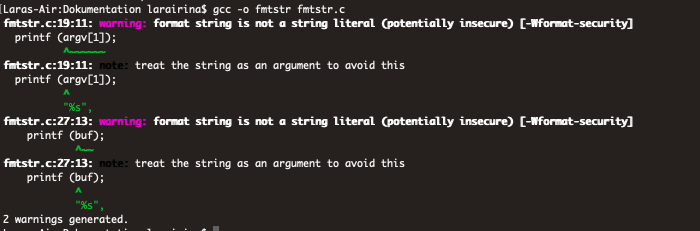
\includegraphics[scale=0.3]{compilation.png}
			\captionof{figure}{Kompilieren des Quellcodes}
			\end{center}
		\item Einfaches Ausführen des Programms ohne Kommandozeilenargumente führt zu folgender Ausgabe:
		\begin{center}
			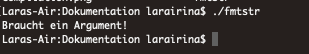
\includegraphics[scale=0.8]{ohneCmdln.png}
			\captionof{figure}{Ausführen des Quellcodes}
		\end{center}
		\item Durch Eingabe zur Laufzeit des unveränderten Programms soll der Wert der Variable \textbf{x} verändert werden
		\item 
		\item
		\item
	\end{enumerate}

	Durch Veränderung der Print-Anweisung in Zeile 30 (siehe Figure 3) ist es einem Angreifer nun nicht mehr möglich dem Compiler einen eigenen Format String zu übergeben und ein Angriff wird so verhindert, da die Variable \textbf{buf} nun nur noch als String, also als Daten-Parameter, interpretiert wird.

\begin{center}
	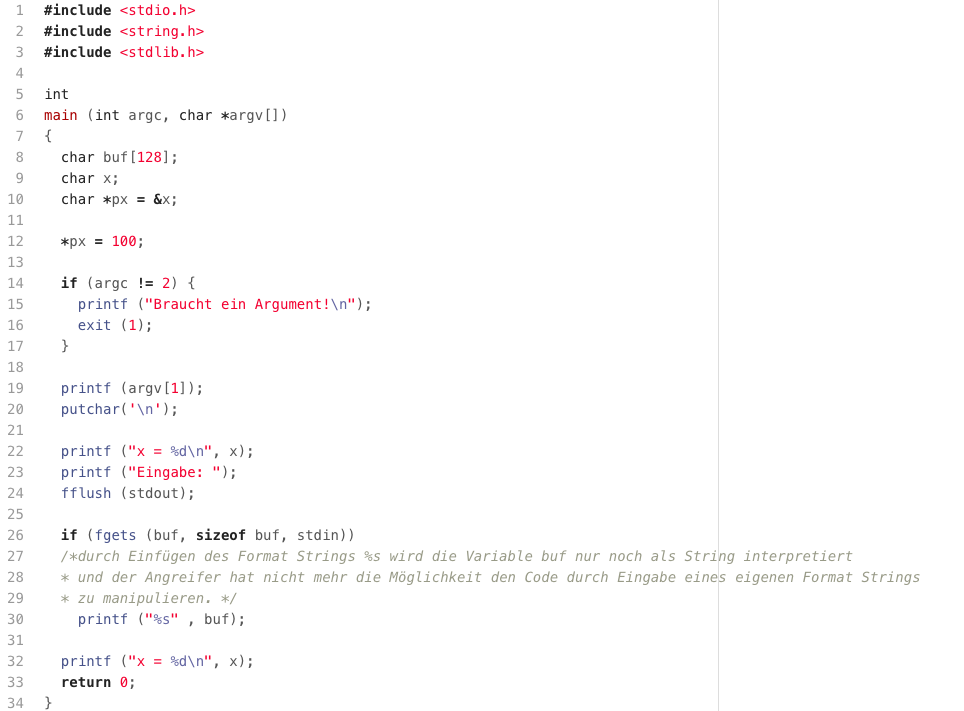
\includegraphics[scale=0.3]{betterCode.png}
	\captionof{figure}{Verbesserter Quellcode}
\end{center}
	
	\section*{Fragen}
	\textbf{Wie kann ein*e Programmierer*in einfach dafür Sorge tragen, dass Format String Angriffe nicht mehr möglich (oder zumindest erheblich erschwert) sind?} \\
	Eine einfache Möglichkeit Format String Angriffe zu verhindern oder erschweren ist die Analyse des Programmcodes. Wird einer Format Funktion wie \textit{printf( )} nur ein Wert übergeben, so kann man davon ausgehen, dass hier ein Angriff möglich ist. Schwachstellen werden so effizient vermieden und die Analyse lässt sich auch automatisiert ausführen. Trotz aller Einfachheit ist hierbei zu beachten, dass ausreichende Programmierkenntnisse notwendig sind um Patches zu erstellen und Quellcodes zur manuellen Analyse häufig zu komplex sind. 
	\bigskip

	Eine weitere Möglichkeit zur Prävention ist das Prüfen auf Speichergrenzen von Variablen während der Programmausführung. So können Buffer Overflows während der Laufzeit erkannt und Angriffe vermieden werden. Um diese Maßnahme anwenden zu können, muss der Quellcode jedoch überarbeitet werden und auch die Performanz kann darunter leiden.
	\bigskip
	
	\textbf{Wie lässt sich einfach herausfinden, ob ein derartiger Angriff vermutlich möglich ist?} \\
	Durch eine Analyse des Quelltextes lässt sich einfach herausfinden, ob ein Format String Angriff möglich ist. Hierbei gilt es herauszufinden, wie viele Werte einer Funktion der printf( )-Familie übergeben werden. Bekommt die Funktion nur einen Wert übergeben, so wird dies ials eine Art benutzerdefiniertes Format interpretiert. Werden jedoch mehr als ein Wert übergeben, so ist davon auszugehen, dass die Format Strings fest vorgegeben sind und ein derartiger Angriff nicht möglich ist. 
	\bigskip
	
	
\end{document}